\documentclass{beamer}
\usepackage[english,russian]{babel}
\usepackage[utf8]{inputenc}
\usepackage{amsmath}
\usepackage{hyperref}
\usetheme{Warsaw}
\usepackage{listings}
\usepackage{xcolor}
\usepackage{tikz}
\usetikzlibrary{graphs}
\usepackage{algpseudocode}

\lstset{
    frame=tb,
    tabsize=4,
    showstringspaces=false,
    numbers=left,
    commentstyle=\color{green},
    keywordstyle=\color{blue},
    stringstyle=\color{red},
    emph={baz},
    emphstyle=\textbf
}

\begin{document}

\title{SAT/SMT solvers\newline 4. Equalities and Uninterpreted Functions}
\author{Roman Kholin}
\institute{Lomonosov Moscow State University}
\date{Moscow, 2023}

\begin{frame}
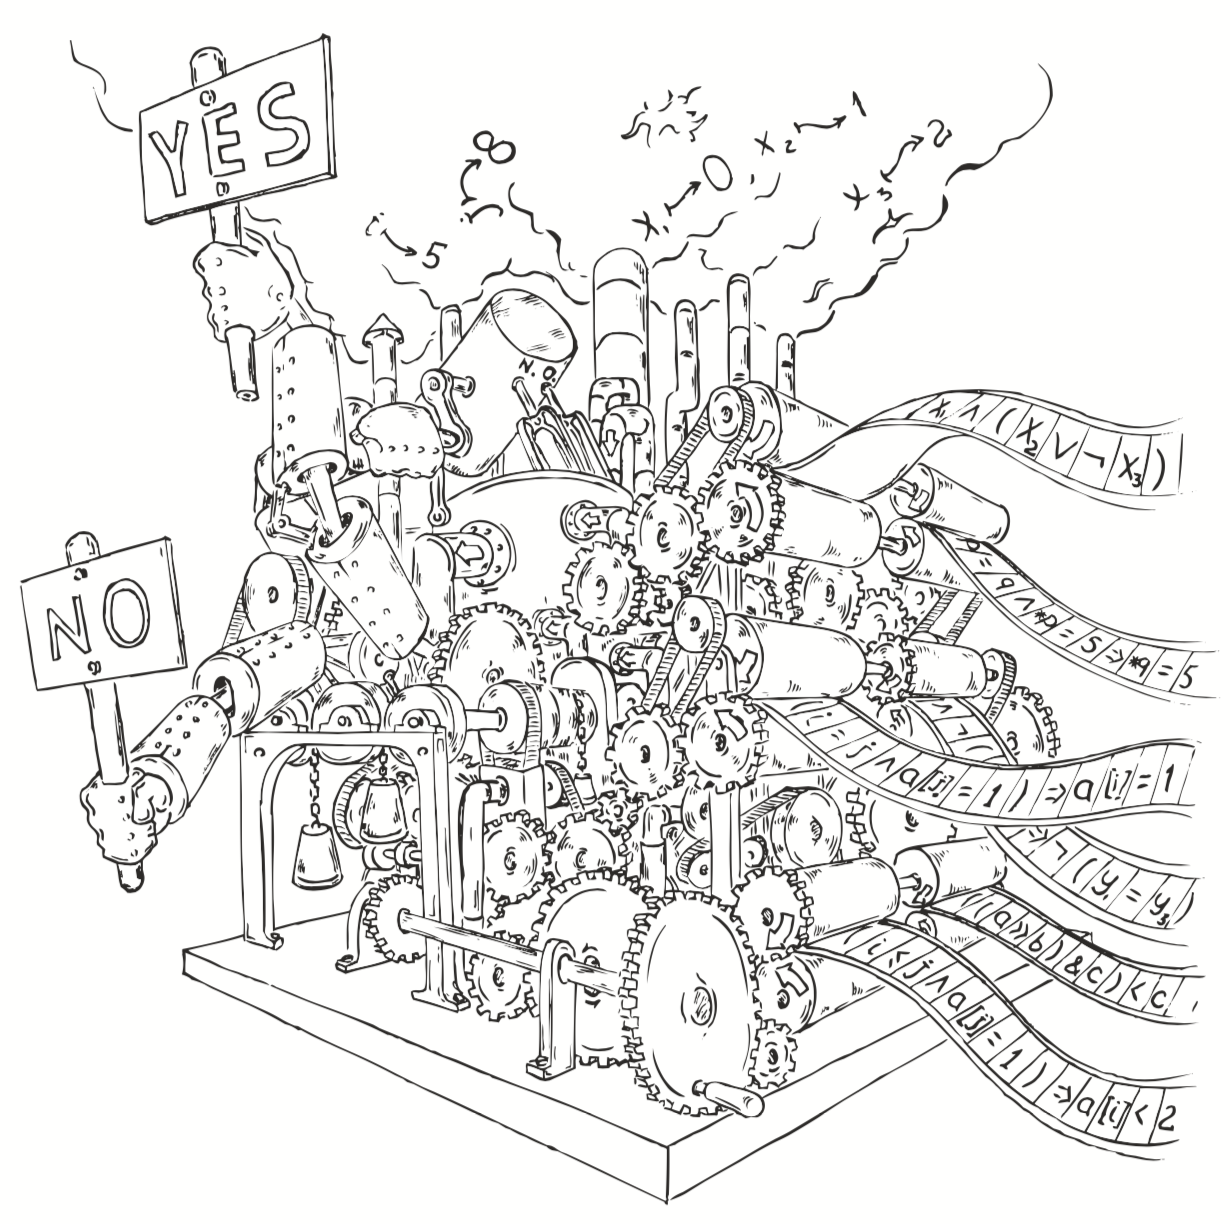
\includegraphics[scale=0.5]{../decision-procedure.png}
\end{frame}

\frame{\titlepage}

\begin{frame}{Definitions}
\begin{block}{Equality logic}
An equality logic formula is defined by the following grammar:
\begin{itemize}
\item $formula: formula \wedge formula$ | $\lnot formula$ | $(formula)$ | $atom$
\item $atom : term = term$
\item $term : identifier$ | $constant$
\end{itemize}
where the identifier s are variables defined over a single infinite domain such as the Reals or Integers. Constants are elements from the same domain as the identifiers.
\end{block}
\end{frame}

\begin{frame}{Removing the constants}
\begin{block}{Theorem}
Given an equality logic formula $\varphi^E$, there is an algorithm that generates an equisatisfiable formula $\varphi^{E'}$ without constants, in polynomial time.
\end{block}
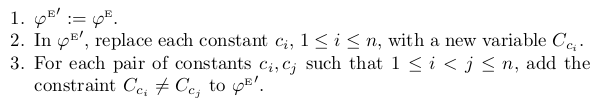
\includegraphics[scale=0.5]{Removing_constants.png}
\end{frame}

\begin{frame}{Definitions}
\begin{block}{Equality logic with Uninterpreted Functions (EUF)}
An equality logic formula with uninterpreted functions and uninterpreted predicates is defined by the following grammar:
\begin{itemize}
\item $formula: formula \wedge formula$ | $\lnot formula$ | $(formula)$ | $atom$
\item $atom : term = term$ | $predicate$-$symbol$ (list of terms)
\item $term : identifier$ | $predicate$-$symbol$ (list of terms)
\end{itemize}
\end{block}
$F(x) = F(G(y)) \vee x + 1 = y$\newline
$F(x) = F(G(y)) \vee PLUS(x, 1) = y$\newline
\begin{block}{Functional consistency}
Instances of the same function return the same value if given equal arguments\newline
$\vDash \varphi^{UF} \Rightarrow \vDash \varphi$
\end{block}
\end{frame}

\begin{frame}{Equivalence of programs}
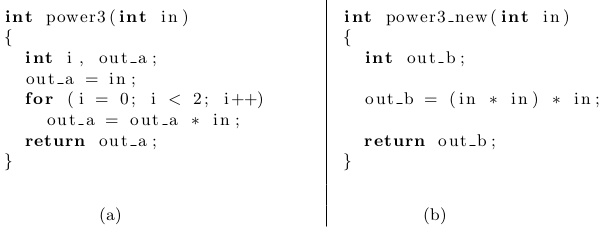
\includegraphics[scale=0.5]{power3.png}
\end{frame}

\begin{frame}{Equivalence of Programs}
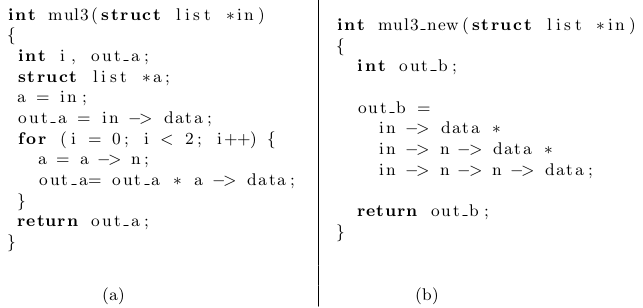
\includegraphics[scale=0.5]{mul3.png}
\end{frame}

\begin{frame}{Equivalence of Programs}
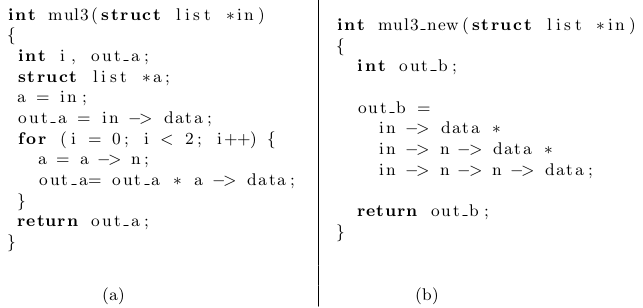
\includegraphics[scale=0.5]{mul3.png}
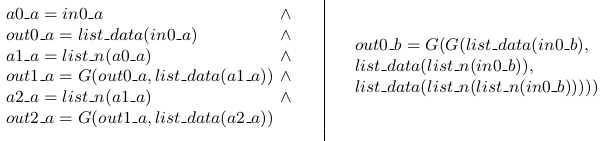
\includegraphics[scale=0.5]{mul3_ans.png}
\end{frame}

\begin{frame}{Congruence closure}
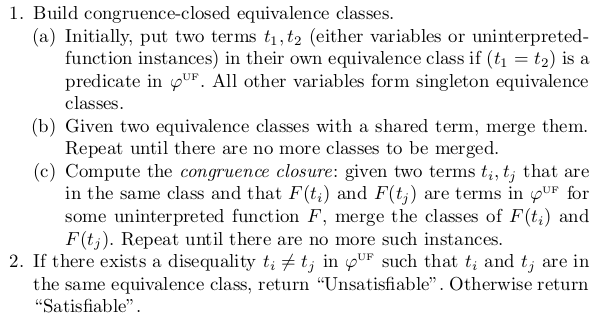
\includegraphics[scale=0.5]{Congruence_closure.png}
\end{frame}

\begin{frame}{Example}
$(x_1 = x_2) \wedge (x_2 = x_3) \wedge (x_4 = x_5) \wedge (x_5 \neq x_1) \wedge (F(x_1) \neq F(x_3))$
\end{frame}

\begin{frame}{Functional consistency is Not Enough}
$(x_1 = y_2) \wedge (x_2 = y_1) \rightarrow (x_1 + y_1) = (x_2 + y_2)$
\end{frame}

\begin{frame}{Functional consistency is Not Enough}
$(x_1 = y_2) \wedge (x_2 = y_1) \rightarrow (x_1 + y_1) = (x_2 + y_2)$
\begin{block}{Abstraction–refinement loop}
\begin{enumerate}
\item $\varphi' := T(\varphi)$ (T is an abstraction function)
\item If $\varphi$ is valid then return <<Valid>>
\item If $\varphi'$ = $\varphi$ then return <<Not valid>>
\item Refine $\varphi$ by adding more constraints or by replacing uninterpreted functions with their original interpreted versions
\item Return to step 2
\end{enumerate}
\end{block}
\end{frame}

\begin{frame}{Examples}
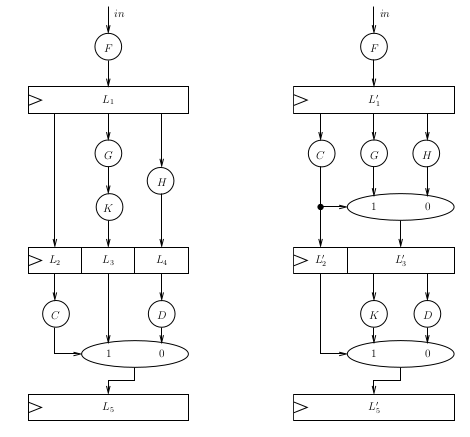
\includegraphics[scale=0.5]{circuit.png}
\end{frame}

\begin{frame}{Examples}
$z = (x_1 + y_1) * (x_2 + y_2)$\newline
$u_1 = x_1 + y_1; u_2 = x_2 + y_2; z = u_1 * u_2$
\end{frame}

\begin{frame}
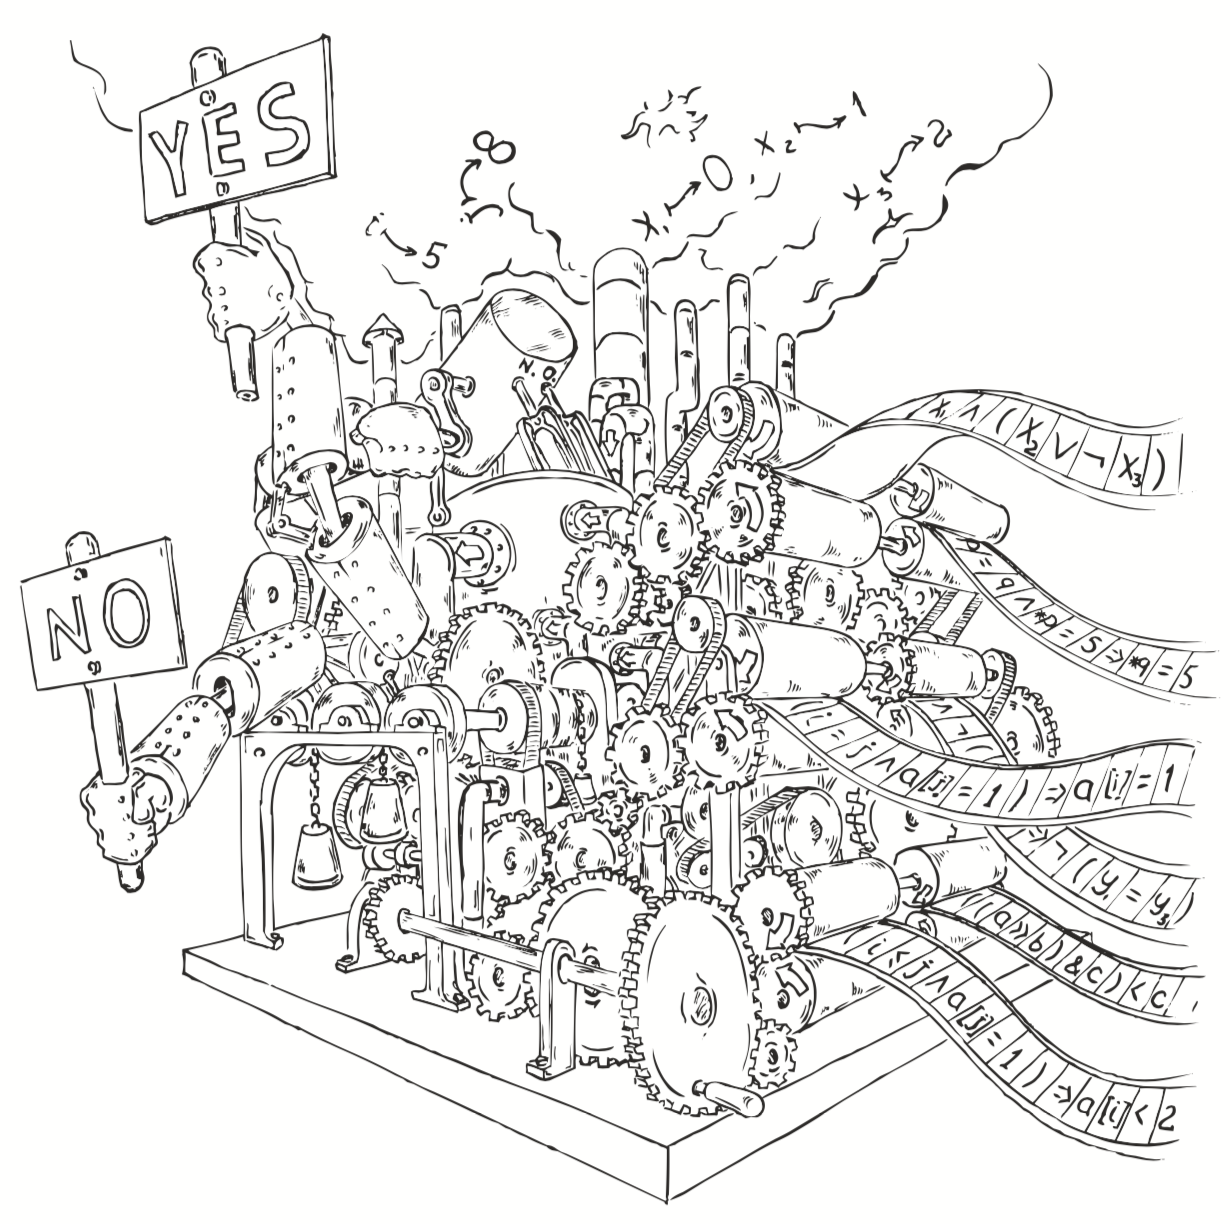
\includegraphics[scale=0.5]{../decision-procedure.png}
\end{frame}

\end{document}
